\glspl{MSR} possess unique characteristics which render existing \gls{LWR}
analysis software inappropriate for \gls{MSR} analysis. Legacy \gls{LWR}
software typically scale poorly on modern high-performance computing
clusters and do not support complex geometries beyond regular \gls{LWR} fuel
assembly lattices. Furthermore, \glspl{MSR} feature strong multiphysics
coupling which force segregated solvers into taking smaller timesteps to
maintain accuracy. This chapter provides a brief history of \glspl{MSR}
development and operation, followed by a discussion of the challenges in
\gls{MSR} multiphysics modeling
for reactor accident analysis. Next, this chapter presents a literature
review of existing multiphysics simulation software developed for \glspl{MSR}
analysis. This work focuses on software for analysing short-term reactor
dynamics which requires the ability to accurately simulate various transient
scenarios such as reactor start-up and coast-down, load-following operations,
steady-state operation, and accident analysis. Long-term dynamics such as fuel
burnup and structural corrosion fall outside the scope of this work. Lastly,
this chapter provides a literature review of turbulence modeling and control
rod modeling, and their relevance in \glspl{MSR} modeling.

\section{Molten Salt Reactors}

\subsection{Historical Molten Salt Reactor Development and Operation}

\gls{ORNL} researchers first conceived the \gls{MSR} concept in pursuit of a
liquid fuel reactor for the US Aircraft Nuclear Propulsion program in
the 1950s \cite{rosenthal_molten-salt_1970}. Due to high temperature
requirements, water-cooled reactors were not suitable as aircraft jet engines
\cite{dolan_1_2017}. Instead, the researchers selected molten fluoride
salts in particular for high uranium solubility, chemical stability, low vapor
pressure even at high temperatures, good heat transfer properties,
resistance against radiation damage, and reduced corrosive effects on some
common structural material \cite{rosenthal_molten-salt_1970}. They
subsequently built the first ever operational \gls{MSR}, 2.5 MW$_{\text{th}}$
\gls{ARE} reactor at \gls{ORNL}. The \gls{ARE}
achieved criticality on November 1954 and generated 100 MWh over nine days.
The reactor ran on enriched uranium in a molten salt mixture of NaF,
ZrF$_4$, and UF$_4$ with BeO neutron moderators. The aircraft program
ultimately never came to fruition as the development of intercontinental
ballistic missiles effectively eliminated the need for long-range
nuclear-powered bomber aircraft.

However, the successful demonstration of the \gls{ARE} spurred further
research into adapting \glspl{MSR} for civilian power generation
\cite{rosenthal_molten-salt_1970}. One key finding from the
research was that the thorium fuel cycle had a better breeding ratio than the
$^{238}$U-to-$^{239}$Pu fuel cycle in thermal-spectrum reactors.
Ultimately, these efforts culminated in the design, construction, and
successful operation of the \gls{MSRE}. The \gls{MSRE} had a 8 MW$_{\text{th}}$,
graphite-moderated design with a LiF-BeF$_2$-ZrF$_4$-UF$_4$ fuel salt mixture
\cite{haubenreich_experience_1970}. In January 1969, the \gls{MSRE} became the
first reactor to run on $^{233}$U fuel bred from $^{232}$Th.

Building on their experience with the \gls{MSRE}, \gls{ORNL} proposed a
new program for the construction and operation of a demonstration reactor
based on the \gls{MSBR} concept that they had
developed \cite{macpherson_molten_1985}. The \gls{MSBR} is a thermal-spectrum,
single fluid reactor with fertile $^{232}$Th isotopes mixed directly into the
FLiBe molten salt for $^{233}$U breeding \cite{robertson_conceptual_1971}. Like the
\gls{MSRE}, the \gls{MSBR} relies on continuous online reprocessing to add
fertile material and remove fission product neutron poisons. Researchers
estimated the doubling time (the minimum amount of time required to produce
enough fissile material to start up another \gls{MSBR}) to be
approximately 22 years. While \gls{ORNL} failed to secure funding for the
\gls{MSBR} program, two independent
technology evaluation and design studies of the \gls{MSR} had reported
favorably on the promise of the system \cite{macpherson_molten_1985}.

Following a relative lull lasting until the late 20th century, researchers at \gls{CNRS} began
research into \glspl{MSR} in 1997 \cite{heuer_simulation_2010}. Starting from the \gls{MSBR}
design, they performed parametric studies on reactor safety, breeding, and other performance
metrics \cite{mathieu_thorium_2006}. They found that graphite-moderated designs required careful
consideration of the fuel-to-moderator ratio as some designs exhibited positive temperature
feedback coefficients. Safer reactor configurations generally operated at very thermalized spectra
owing to large neutron losses in the graphite, or at epithermal and fast spectra owing to
$^{232}$Th resonance capture cross sections. Combined with findings on poor breeding performance
with thermal spectra and accelerated graphite irradiation damage with fast spectra, the authors
suggested eliminating the graphite moderator to optimize both reactor safety and breeding.

Their efforts culminated in the \gls{MSFR} concept, a fast-spectrum breeder \gls{MSR}
designed to run on the thorium fuel cycle \cite{merle_optimized_2007}. As opposed to the
multi-channel design of the \gls{MSRE} and \gls{MSBR}, the \gls{MSFR} reactor core consists of a
single, large channel through which the salt flows as shown in Figure \ref{fig:msfr}. In 2008, the
Generation IV International Forum highlighted the \gls{MSFR} among other \gls{MSR} designs for
further development \cite{gif_generation_2008}. The \gls{MSFR} has also benefited from
collaborative research through three projects, the \gls{EVOL} \cite{euratom_final_2015},
\gls{SAMOFAR} \cite{kloosterman_20_2017}, and \gls{SAMOSAFER} \cite{cordis_severe_nodate} projects.
Under the \gls{EVOL} project, researchers further optimized the \gls{MSFR} design based on
neutronic and thermal-hydraulic safety analyses. One significant modification involved a transition
from the original straight cylinder core design to curved walls in the reactor core to facilitate
smoother fuel salt flow and prevent large eddies from forming in the core
\cite{rouch_preliminary_2014}. Large eddies create hot, swirling pockets of fuel salt which could
complicate reactor operation. For instance, changes in flow conditions, intended or otherwise,
could cause the eddies to collapse and in turn introduce a localized pocket of hot fuel salt to the
circulating fuel loop. Coupled with the strong temperature reactivity feedback in the \gls{MSFR},
reactor could experience large power fluctuations every time the hot fuel salt passes through the
core. The \gls{SAMOFAR} project, which started approximately two years after the end of the
\gls{EVOL} project, supported more comprehensive safety assessments of the reactor and the
reprocessing plant, and funded a number of experiments for validation of the \gls{MSFR}'s safety
features. The ongoing \gls{SAMOSAFER} project funds further research activities with the goal of
achieving modeling, analysis, and design improvements on various aspects of \gls{MSR} operation and
safety.
%
\begin{figure}[htb!]
	\centering
	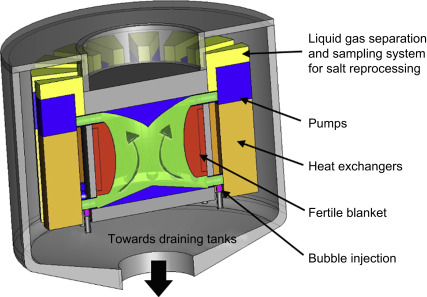
\includegraphics[width=.7\columnwidth]{msfr}
	\caption{Schematic diagram of the \gls{MSFR}. Retrieved from 
	\cite{allibert_7_2016}.}
	\label{fig:msfr}
\end{figure}

China and India have also started national programs supporting \gls{MSR}
development. China launched their \gls{TMSR} program in 2011 to develop and
construct both solid-fueled and liquid-fueled \gls{TMSR} designs
\cite{zou_research_2019}. Latest updates at the time of writing indicate that a
2-MW liquid-fueled prototype will complete construction by August
2021, with tests expected to start the following month. India also signaled
their interest especially in thorium-based
reactors given their vast thorium reserves
\cite{jayaram_overview_1987}. They have developed conceptual designs of the
\gls{IMSBR}, expected to run on a fast/epithermal neutron spectrum to avoid
using graphite moderators given their tendency to deform under high neutron
fluence.

In the US, Southern Company received funding from \gls{DOE}'s
\gls{ARDP} \cite{doe_office_2021} to design, construct, and operate the
\gls{MCRE}, a prototype chloride salt-based \gls{MSR} relevant to TerraPower's
\gls{MCFR} \cite{terrapower_mcfr_2020}. This project builds on a prior
five-year cost-sharing project for the development of the \gls{MCFR} involving
TerraPower, Southern Company, Oak Ridge National Laboratory, Idaho National
Laboratory, the Electric Power Research Institute, and Vanderbilt University.
The \gls{MCFR} is a fast-spectrum \gls{MSR} similar to the \gls{MSFR}.
Canada-based Terrestrial Energy is also developing their \gls{IMSR}
\cite{leblanc_18_2017}, a small modular \gls{MSR} based on the \gls{MSRE}. The
replaceable \gls{IMSR} core-unit which holds the reactor core, pumps, heat
exchangers, and control rods, runs for approximately 7 years before it is shut
down and replaced after a cool-down period.

With the renewed global interest in \glspl{MSR}, \gls{MSR} modeling software play an important role
in supporting \gls{MSR} development. Reactor modeling can accelerate reactor design and
optimization by enabling engineers to iterate through numerous design changes. \gls{MSR} modeling
software are also essential tools in reactor safety analysis and licensing efforts as engineers
must demonstrate and verify their \gls{MSR} designs remain safe under various accident scenarios.
However, many reactor software were tailored for modeling solid-fueled reactors such as \glspl{LWR}
which make up most of the world's operating reactor fleet. \glspl{MSR} possess unique features and
physics which are typically not modeled in other reactor types. The \gls{ARE} and \gls{MSRE}
projects first demonstrated the feasibility of a liquid-fueled reactor with fissile fuel dissolved
in the molten salt coolant. The \gls{MSBR} design features $^{233}$U breeding from $^{232}$Th with
online fuel reprocessing as opposed to batch-wise reprocessing of solid-fueled breeder reactors.
The various modern \gls{MSR} designs feature numerous changes relative to the older \gls{MSRE} and
\gls{MSBR} designs such as running on epithermal and fast neutron spectrums, different core
structures, and different molten salt compositions.

\gls{MSR} modeling software play an important role in supporting
\gls{MSR} development. They accelerate reactor design and optimization by
enabling engineers to iterate through numerous design changes. \gls{MSR}
modeling software are also essential tools in reactor safety analysis and
licensing efforts as engineers must demonstrate and verify their \gls{MSR}
designs remain safe under various accident scenarios. The next section
identifies challenges in \gls{MSR} multiphysics modeling with respect to
reactor accident analysis.

\section{Challenges in MSR Multiphysics Modeling} \label{sec:challenges}

While modeling \glspl{MSR} is not necessarily more difficult than modeling
solid-fueled reactors, we must adapt our software tools to accurately model the
unique phenomena found in these circulating-fuel reactors. The differences in
the challenges of simulating \glspl{MSR} compared to solid-fueled reactors stem
mainly from the liquid fuel form of the fuel salt \cite{huff_identifying_2019,
diamond_phenomena_2018}.

Firstly, liquids generally exhibit greater thermal
expansion per unit change in temperature than solids. A decrease in density of
the fuel medium increases the likelihood of neutrons escaping the fuel region
and being absorbed by non-fissile material elsewhere in the reactor.
Consequently, combined with the temperature-dependent Doppler broadening of
resonance capture cross sections, \glspl{MSR} possess stronger negative fuel
temperature reactivity feedback than their solid-fueled counterparts
\cite{elsheikh_safety_2013}. These
phenomena ultimately result in strong interactions between the neutron fluxes
and core temperatures given that neutron fluxes affect core temperatures
through fission heat generation and core temperatures in turn affect neutron
fluxes through the mechanisms as described prior.

Secondly, with the fuel
salt also serving the role of providing cooling in the core, velocity flow
profiles in the fuel salts strongly impact the temperature distribution via
advection-dominated heat transfer \cite{diamond_phenomena_2018}. This contrasts
with the relatively static temperature distribution shapes in fuel pins and
other forms of solid fuel matrixes physically separated from the coolant; 
changes in coolant and the resultant changes in heat transfer rates in
solid-fueled reactors are often reduced to empirical correlations governing
convective heat transfer between the fuel cladding and the coolant. On the
other hand, the velocity flow profile has a more direct effect on the
temperature distribution and the temperature-dependent neutron cross sections
in \glspl{MSR}.

Lastly, \glspl{DNP} flow freely within the primary coolant loop as opposed to
being held in place as in solid-fueled reactors. Thus, the delayed neutron
source distribution varies significantly depending on the flow profile and
velocity. In addition, the reactor loses some delayed neutrons from out-of-core
\gls{DNP} decay. These delayed neutrons are considered lost as they're emitted
in subcritical regions and are unlikely to contribute to further fission
reactions in the active core. The reduced delayed neutron fraction in the core
contributes to a greater prompt power spike following a reactivity insertion
event compared to solid-fueled reactors, absent any temperature reactivity
feedback. Thus, accurate \gls{MSR} transient simulations require accurate
modeling of \gls{DNP} drift.

As a result, multiphysics
software must employ \textit{tight coupling schemes} to couple the neutronics
and thermal-hydraulics governing equations to accurately capture the strong
multiphysics interactions in transient \gls{MSR} simulations. Tightly coupled
numerical models handle multiphysics interactions by either updating all state
variables simultaneously in one monolithic solve (\textit{full coupling}) or
iteratively updating all state variables (\textit{fixed point iterations})
until the solution converges in every timestep \cite{keyes_multiphysics_2013}.
Full coupling tends to be more computationally expensive because it combines
all physics equations into a single large system of equations to be solved
simultaneously, whereas fixed point iterations involve operator splitting to
separate the system of equations into smaller systems based on their associated
physics, solving smaller systems separately, and iteratively updating the state
variables until convergence. Fixed point iterative methods are often less
stable, less accurate, and have poorer
convergence rates since these methods make iterative corrections
without any regard to potentially destabilizing modes introduced by the
multiphysics coupling \cite{keyes_multiphysics_2013}. Notably, proven
techniques exist for improving the performance of fixed point iteration
coupling schemes for many relevant computational multiphysics research fields,
including reactor analysis \cite{ragusa_consistent_2009}. While fully coupled
schemes deal with solving a large system of equations, they can outperform
fixed point iterative methods in some multiphysics problems through superior
stability and convergence rates. 

In contrast to tight coupling schemes, \textit{loose coupling schemes}
solve each set of single-physics equations using state variable
data from the previous timestep without iterative corrections within every
timestep. Loosely coupled schemes are inappropriate for modeling \glspl{MSR}
given the strong coupling between the neutronics and thermal-hydraulics.
Aufiero et al. \cite{aufiero_development_2014} demonstrated a loose coupling
approach that failed to reproduce the expected increase in reactor power
in an \gls{MSR} in response to a 150 pcm reactivity insertion.

Consequently, most MSR multiphysics simulation tools employ, at
the very least, tight coupling schemes through fixed point iterations. The
next section explores various numerical coupling approaches in existing
multiphysics \gls{MSR} simulation tools.

\section{MSR Multiphysics Simulation Tools} \label{sec:msr-tools}

In recent years, several simulation tools have been developed for full-core
modeling of fast-spectrum \glspl{MSR}. \textit{Tightly coupled} approaches,
through segregated solvers, involve coupling separate single-physics neutronics
and thermal-hydraulics software. For example, researchers at
the \gls{TUD} coupled the 3D neutron diffusion software DALTON
\cite{boer_validation_2010} and the \gls{CFD} software HEAT
\cite{de_zwaan_static_2007} to perform a safety analysis of the \gls{MSFR}
\cite{fiorina_modelling_2014}. In a later effort from the same institute,
Tiberga et al. \cite{tiberga_discontinuous_2019} coupled PHANTOM-$S_N$ and
DGFlows in their participation in the CNRS benchmark study
\cite{tiberga_results_2020}. The CNRS benchmark, named after the \gls{CNRS}
where it was originally developed, facilitates code-to-code verification of
\gls{MSR} multiphysics software \cite{aufiero_testing_2018}. Another
multiphysics package was developed at the Paul Scherrer Institute (PSI)
coupling the thermal-hydraulics system software \gls{TRACE}
\cite{nrc_trace_2007} with the
nodal neutron diffusion software \gls{PARCS} \cite{downar_parcs_2010} for the
safety analysis of the \gls{MSFR} \cite{pettersen_coupled_2016}. Coupling
single-physics software to form an integrated multiphysics tool allows
researchers to leverage on older, well-validated, single-physics software.
These single-physics software are also highly optimized for solving specific
types of \glspl{PDE} relevant to the investigated system.

With modern advancements in computing hardware and growing access to
high-performance computing systems, others have developed multiphysics tools by
coupling the \gls{CFD} software OpenFOAM
\cite{the_openfoam_foundation_ltd_openfoam_2021} with the Monte Carlo particle
transport software
Serpent \cite{leppanen_serpent_2014}, thus achieving high-fidelity neutronics
calculations in transient reactor analyses. Laureau et al.
\cite{laureau_transient_2017} developed an innovative technique called the
\gls{TFM} method through the introduction of additional time-dependence
operators to conventional fission matrices typically used to accelerate source
convergence in Monte Carlo neutronics calculations. The \gls{TFM} method
pre-calculates three \glspl{TFM} of the reactor system in Serpent and
interpolates the matrix values during the actual transient calculations to
incorporate the effects of temperature-induced density change and Doppler
effect on the neutron cross sections and ultimately the neutron flux. Blanco
\cite{blanco_neutronic_2020} took a more integrated approach by
compiling Serpent as an internal \texttt{C}-based function within OpenFOAM's
\texttt{C++}-based framework. This approach reduced the amount of required data
transfers between Serpent and OpenFOAM as both software have access to shared
memory during runtime. Their integrated tool employs the Quasi-Static
method for transient neutronics calculations and runs Serpent Monte Carlo
calculations several times per timestep until convergence is reached.

Another \gls{MSR} simulation approach involves developing ``all-in-one''
multiphysics software which handle all multiphysics calculations and data
transfer internally. Among earlier efforts, Nicolino et al.
\cite{nicolino_coupled_2008} and Zhang et al. \cite{zhang_development_2009}
recognized the
need for more robust multiphysics coupling techniques and higher-fidelity
thermal hydraulics solutions to accurately capture complex flow profiles in
pool-type \glspl{MSR}. They each independently developed unnamed multiphysics
simulation tools and demonstrated their tools with non-moderated \gls{MSR}
designs. Later, Li et al. \cite{li_transient_2015} demonstrated the
steady-state and transient analysis capabilities of COUPLE, a neutronics and
thermal-hydraulics software developed at the Karlsruhe Institute of Technology.
Others adopted extensible software frameworks for developing numerical solvers
to develop multiphysics reactor analysis software. Examples of these software
frameworks include the commercial COMSOL
Multiphysics\textsuperscript{\textregistered} software
\cite{comsol_ab_comsol_nodate}, the aforementioned open-source CFD toolbox
OpenFOAM, and the open-source finite-element
framework \gls{MOOSE} \cite{gaston_physics-based_2015}. Researchers at
\gls{PoliMi} developed a \gls{MSR} simulation tool in COMSOL and
modeled the \gls{MSBR} as a single axisymmetric fuel channel with a uniform
flow profile \cite{cammi_multi-physics_2011}, followed by the \gls{MSRE} core
also as a single axisymmetric fuel channel with parabola-shaped laminar flow
\cite{cammi_dimensional_2012}. They later expanded on their approach by
modeling the \gls{MSRE} upper plenum, downcomer and lower plenum, primary heat
exchanger, and secondary heat exchanger as 0D systems (lumped-parameter model),
and substituting the 2D fuel channel with a 3D fuel channel which more closely
resembled the actual fuel channels in the \gls{MSRE}
\cite{zanetti_geometric_2015}. Beyond graphite-moderated \glspl{MSR}, they
also modeled the \gls{MSFR} in the same publication which featured \gls{TUD}'s
DALTON + HEAT coupled multiphysics tool.
More recently, several European institutes (\gls{CNRS}, \gls{PoliMi},
and the \gls{PSI}) have also developed coupled neutronics and
thermal-hydraulics tools in OpenFOAM. Their tools share some
similarities such as implementing the $SP_N$ simplified $P_N$ neutron transport
model and leveraging OpenFOAM's turbulent flow modeling capabilities.
Differences include fuel compressibility modeling and helium bubble tracking
capabilities from \gls{PoliMi} \cite{cervi_development_2019}, fuel
performance analysis capability from \gls{PSI} \cite{fiorina_creation_2018},
and the aforementioned external coupling capability with Serpent from
\gls{CNRS} \cite{blanco_neutronic_2020}.

Finally, within the MOOSE framework, simulation tools capable of modeling
\glspl{MSR} include: Rattlesnake \cite{wang_rattlesnake_2021}; and Moltres
\cite{lindsay_moltres_2017}\textemdash the subject of this work.
Rattlesnake primarily tackles radiation transport problems, but the MOOSE
framework facilitates multiphysics coupling
with MOOSE-based applications for other physics
such that all applications share the same data structure. This eliminates
computational costs from external data transfers and optionally allowing for
\textit{fully coupled} solves in which the application solves all physics
simultaneously. Similarly, Moltres benefits from the highly-integrated
cross-compatibility
within the ecosystem of MOOSE-based applications. Abou-Jaoude et al.
\cite{abou-jaoude_coupled_2020} coupled Rattlesnake with Pronghorn, another
MOOSE-based application for advanced reactor thermal-hydraulics modeling, to
demonstrate several steady-state \gls{MSR} simulation capabilities defined in
the CNRS benchmark. Lindsay et al.
\cite{lindsay_introduction_2018} first demonstrated Moltres' \gls{MSR} modeling
capabilities on 2D axisymmetric and 3D Cartesian models of the \gls{MSRE} with
fixed velocity flow on a fully coupled neutronics and thermal-hydraulics solve.
We later demonstrated some of Moltres' more recent developments through
modeling a 2D axisymmetric model of the \gls{MSFR} for steady-state operation
and transient accident analysis \cite{park_advancement_2020}. The latter study
introduced looped \gls{DNP} flow, coupling the \gls{DNP} drift and temperature 
advection-diffusion to incompressible flow, and decay heat modeling
capabilities. The proposed work aims to continue Moltres development for
multiphysics \gls{MSR} analysis. Chapter \ref{chap:moltres} describes Moltres
and its existing capabilities for reactor analysis.

\section{Turbulence Modeling in MSRs}

In fluid dynamics, turbulent flow is characterized by unsteady, irregular, and
chaotic fluid motion as opposed to neat, parallel flow layers in laminar flow
\cite{pope_turbulent_2000}. The transition from laminar to turbulent flow
typically occur at Reynolds numbers between 2000 and 4000, depending on the
setup \cite{pope_turbulent_2000}. Turbulent flows are expected in \glspl{MSR}.
Kedl \cite{kedl_fluid_1970} reports expected Reynolds numbers in the \gls{MSRE}
ranging from 1000 in the regular fuel coolant channels to over 10000 in the
flow distributor volute and core wall cooling annulus regions. For the
\gls{MSFR}, salt flow in the central core region is highly turbulent and
reaches Reynolds numbers on the order of $10^5$.

\subsection{Turbulence Models}

Numerous types of turbulence models exist for various turbulent flow
applications. The most common turbulence models can be classified into the
following categories by order of increasing computational complexity:
%
\begin{itemize}
    \item \gls{RANS}-based models
    \begin{itemize}
        \item Eddy viscosity models
        \begin{itemize}
            \item Algebraic models
            \item One- and two-equation models
        \end{itemize}
        \item \gls{RSM}
    \end{itemize}
    \item \gls{DES}
    \item \gls{LES}
    \item \gls{DNS}
\end{itemize}

\gls{RANS}-based models are based on the \gls{RANS} equations obtained from
applying time-averaging to the equations of fluid flow. The \gls{RANS}
equations separate flow into time-averaged $U$ and fluctuating $u$ components
and can be writtin in Einstein notation and Cartesian coordinates as:
%
\begin{align}
    \frac{\partial U_i}{\partial t} + U_j \frac{\partial u_i}{\partial x_j} =&
    -\frac{1}{\rho} \frac{\partial P}{\partial x_i} + \nu \nabla^2 U_i -
    \frac{\partial \langle u_i u_j \rangle}{x_j}
    \shortintertext{where}
    \langle \cdot \rangle =& \mbox{ time-averaging operator,} \nonumber \\
    \rho =& \mbox{ fluid density,} \nonumber \\
    P =& \mbox{ time-averaged pressure field,} \nonumber \\
    \nu =& \mbox{ kinematic viscosity.} \nonumber
\end{align}

Eddy viscosity models, which comprise of the most widely used turbulence models
in use today \cite{rodi_turbulence_2017}, operate on the eddy viscosity
hypothesis which states that the Reynolds stresses in the \gls{RANS} equations
are given by:
%
\begin{align}
    \langle u_iu_j \rangle =& \frac{2}{3}k \delta_{ij} - \nu_T \left(
    \frac{\partial U_i}{\partial x_j} + \frac{\partial U_j}{\partial x_i}
    \right)
    \shortintertext{where}
    k =& \mbox{ mean turbulent kinetic energy,} \nonumber \\
    \delta_{ij} =& \mbox{ Kronecker delta,} \nonumber \\
    \nu_T =& \mbox{ eddy viscosity.} \nonumber \\
\end{align}

The various eddy viscosity models mainly differ in their approach towards
the closure problem of calculating the eddy viscosity. As the name suggests,
algebraic models rely on algebraic equations to calculate the eddy viscosity
distribution directly from flow variables. As a result, algebraic models are
the least computationally intensive models for turbulence. Algebraic models
can be further categorized into two types: uniform eddy viscosity models
and mixing length models. Uniform eddy viscosity models apply a uniform eddy
viscosity throughout the problem domain. The uniform eddy viscosity is
calculated from flow parameters such as the characteristic velocity, the
characteristic flow width, and empirically determined turbulent Reynolds
number. Given that eddy viscosities usually vary significantly in most types of
flow, uniform eddy viscosity models have a very limited range of applicability
\cite{pope_turbulent_2000}. Mixing length models add a level of complexity by
relating the eddy viscosity to spatially-varying flow parameters such as the
mean velocity gradient (Prandtl \cite{prandtl_7_1925} and Cebeci-Smith
\cite{smith_numerical_1967} models) or the mean rate of strain (Baldwin-Lomax
\cite{baldwin_thin-layer_1978} model) and an empirical mixing length parameter.
Combined with empirical data for the mixing length parameter, these
models provide better approximations of free shear flows, but still
underperform for more complex flows involving flow separation and significant streamline curvature.

One- and two-equation turbulence models introduce differential equations to
describing turbulence quantities such as the turbulence kinetic energy and the
turbulence rate of dissipation to obtain the eddy viscosity distribution. The
most common and best performing one-equation model is the Spalart-Allmaras
model which provides an equation for the eddy viscosity directly with several
closure coefficients and functions \cite{wilcox_turbulence_2006}. The
Spalart-Allmaras model is considered ``complete'' as it does not involve any
adjustable coefficients or functions. Calibrated for free shear flows in
aeronautical applications, the model performs modestly better than algebraic
models in these applications \cite{pope_turbulent_2000}, but it still deviates
significantly from experimental data
for separated flows \cite{wilcox_turbulence_2006}.

Investigations with
one-equation models reveal the need for an extra equation to account for
turbulent length scales separately from turbulent velocity. Thus, two-equation
models became the most widely adopted turbulence model in the late 20th century
\cite{pope_turbulent_2000}. Two-equation models include the $k$-$\epsilon$,
$k$-$\omega$, and $k$-$\tau$ models. The variables $k$, $\epsilon$, $\omega$,
and $\tau$ correspond to turbulent kinetic energy, turbulent dissipation,
specific turbulent dissipation rate, and turbulent time scale, respectively.
While none of these models perform universally well, they are generally more
accurate than the algebraic and one-equation models. Successive contributions
and modifications to the two-equation models through the years have also
improved their performance in predicting various types of turbulent flow. Their
moderate computational expense compared to expensive, high-fidelity turbulence
models favor their adoption in most commercial \gls{CFD} software for
engineering applications \cite{pope_turbulent_2000}.

\glspl{RSM} directly computes the individual components $\langle u_i u_j
\rangle$ of the Reynolds stress tensor instead of approximating it with a
single, isotropic eddy viscosity term. As a consequence, \glspl{RSM} provide
more realistic predictions for flows with significant rotational motion and
sudden changes in the mean strain rate, albeit at greater computational
expense, compared to the one- and two-equation models
\cite{wilcox_turbulence_2006}. Smaller improvements are observed in modeling
free shear flows and backward-facing step flows \cite{wilcox_turbulence_2006}.

Due to the much higher computational cost for \gls{DES}, \gls{LES}, and
\gls{DNS}, these models have limited applicability in routine, high-Reynolds
number engineering problems today. However, given their high accuracy, these
models are useful for flow problems with relatively simple geometries and at
low Reynolds numbers and validating the lower-fidelity turbulence models
\cite{zhiyin_large-eddy_2015}.

\subsection{Turbulence Modeling in MSR Simulation Tools}

For MSR modeling, the $k$-$\epsilon$ and $k$-$\omega$ turbulence models are the
most commonly used models as shown in published work with COMSOL
\cite{fiorina_modelling_2014}, OpenFOAM \cite{aufiero_development_2014}, and
\gls{TUD}'s in-house codes \cite{fiorina_modelling_2014,tiberga_results_2020}.
Podila et al. \cite{podila_cfd_2019} performed \gls{CFD} simulations of the
\gls{MSRE} core with six different turbulence models, namely a Spalart-Allmaras
model, two variants of the $k$-$\epsilon$ model, a $k$-$\omega$ model, and two
variants of \glspl{RSM}. Their results showed relatively small differences
in graphite and fuel temperatures among different turbulence models. However,
they observed significant differences in the turbulence intensities near the
wall. Given the lack of experimental data for model validation, the authors
could not make a clear assessment of the models' accuracies. Nevertheless, the
close agreement of the fuel temperatures imply that the discrepancies in the
turbulent intensities near the wall have a negligible impact on the overall
distribution of advected quantities in the \gls{MSRE}. Podila et al.
\cite{podila_cfd_2019} opted to use a $k$-$\epsilon$ model for subsequent
calculations in their work given its lowest computational cost and the close
agreement in the temperature distributions.

Amongst other \gls{MSR} simulation tools, the $k$-$\epsilon$ and $k$-$\omega$
turbulence models are the most commonly used models as shown in published work
with COMSOL \cite{fiorina_modelling_2014}, OpenFOAM
\cite{aufiero_development_2014}, and \gls{TUD}'s in-house codes
\cite{fiorina_modelling_2014,tiberga_results_2020}. Fiorina et al.
\cite{fiorina_modelling_2014} compared the flow distribution from both models
in a 2D axisymmetric \gls{MSFR} geometry and observed that the $k$-$\omega$
model produced a wider recirculation zone near the outer wall, an additional
recirculation zone near the top wall, and significantly higher maximum
temperatures within the former recirculation zone. Thus, their work highlights
the difficulties of modeling separated flows and calls for extra attention
towards the choice of turbulence model in \glspl{MSR}.

\section{Control Rod Modeling}

Most reactor designs have control rods to control the fission rate or completely shut down the
reactor by inserting the rods further into the reactor core. As such, control rods consist of
strong neutron absorbers like boron, cadmium, and gadolinium to reduce the number of fission
neutrons available to contribute to further fission chain reactions. All reactors start operation
with excess reactivity to ensure that they have enough fissile material to last through to the next
scheduled refueling. Control rods, along with burnable poisons, allow reactors to operate at a
multiplication factor of unity by canceling out the excess reactivity. Control rods are also useful
for ramping the power up or down during start-up, shut-down, or load-following operations. Most
importantly, control rods provide a safety mechanism for quickly shutting down a reactor under
dangerous conditions. Rapid control rod insertion is the main mechanism of a reactor scram to
reliably introduce a large negative reactivity insertion in response to an unintended reactivity
insertion or other events which may threaten the safe operation of the reactor. 

The number and locations of control rods in a reactor vary significantly for different reactor
types, depending on their maximum operating power, refueling frequency, and other factors. For
instance, as shown in Figure *, a single fuel assembly in a \gls{PWR} can accommodate 24 control
rods in close proximity to the fuel pins. The total number of fuel assemblies vary from 37
assemblies in the NuScale VOYGR reactor to 157 assemblies in the Westinghouse AP1000 reactor. On
the other hand, the entire MHTGR-350 high-temperature gas reactor, shown in Figure *, has 30
control rods in total. The control rods are located in graphite reflector blocks, thereby placing
them further from fuel elements. Lastly, the \gls{MSRE} design has three control rods located
centrally in graphite-moderated core with fuel salt channels. While the objective of the proposed
work is to improve diffusion-based control rod modeling in Moltres for \gls{MSR}-like designs, this
literature review also explores existing methods developed for other reactor types.

[Insert control rod illustration]

\subsection{Challenges of Control Rod Modeling} \label{sec:challenges-control-rod}

In reactor design studies, we aim to determine control rod worth which is measured as the reduction
in the neutron multiplication factor $k_{eff}$ due to the presence of the control rod in the
reactor. We are also interested in the accompanying change in flux shape in the vicinity of the
control rod. Neutrons entering the control rods have a higher chance of being absorbed than
adjacent regions in the reactor core. Therefore, control rods induce highly anisotropic neutron
angular fluxes and sharp gradients in the neutron flux in their vicinity. Control rods also cause
shifts in the neutron energy spectrum because their absorption cross sections are much higher in
the lower neutron energy range; more energetic neutrons generally have a higher probability of
escaping the control rod region. As a consequence, modeling control rods accurately requires
high-fidelity computational methods to capture the angular- and energy-dependence in the neutron
flux near the highly absorbing medium.

High-fidelity \textit{neutron transport methods} fall under two categories: stochastic Monte Carlo
methods and deterministic methods. Monte Carlo methods involve simulating a finite number of
neutron histories. Randomly generated numbers determine the outcome of various probabilistic events
such as travel distances between particle collisions, types of collisions, and scattering angles in
each history until it is terminated by a neutron capture event. Deterministic methods for neutron
transport, such as the discrete ordinates $S_N$ and spherical harmonics $P_N$ methods, solve the
\gls{BTE} for neutron transport with some approximations for handling the angular and energy
dependence. The \gls{BTE} for neutron transport is given as:
%
\begin{align}
  \frac{1}{v(E)} \frac{\partial}{\partial t} \Psi(\vec{r},E,\hat{\Omega},&t) + \hat{\Omega}\cdot
  \nabla\Psi(\vec{r},E,\hat{\Omega},t) + \Sigma_t(\vec{r},E,t)\Psi(\vec{r},E,\hat{\Omega},t) 
  \nonumber \\
  - \int^\infty_0 dE'& \int_{4\pi} d\hat{\Omega}' \Sigma_s(\vec{r},E'\rightarrow E,\hat{\Omega}'
  \rightarrow \hat{\Omega},t) \Psi(\vec{r},E',\hat{\Omega}',t) \nonumber \\
  =& \frac{\chi(E)}{4\pi}
  \int^\infty_0 dE' \int_{4\pi} d\hat{\Omega}' \nu\Sigma_f(\vec{r},E',t) \Psi(\vec{r},E',
  \hat{\Omega}',t)+S(\vec{r},E,\hat{\Omega}',t) \label{eq:bte}
  \shortintertext{where}
  v(E) =& \mbox{ neutron velocity,} \nonumber \\
  \Psi(\vec{r},E,\hat{\Omega},t) =& \mbox{ neutron angular flux,} \nonumber \\
  \vec{r} =& \mbox{ spatial coordinates,} \nonumber \\
  E =& \mbox{ neutron energy,} \nonumber \\
  \hat{\Omega} =& \mbox{ direction of neutron travel,} \nonumber \\
  t =& \mbox{ time,} \nonumber \\
  \Sigma_t(\vec{r},E,t) =& \mbox{ macroscopic total cross section,} \nonumber \\
  \Sigma_s(\vec{r},E'\rightarrow E,\hat{\Omega}'\rightarrow \hat{\Omega},t) =&
  \mbox{ macroscopic scattering cross section,} \nonumber \\
  \chi(E) =& \mbox{ fission neutron spectrum,} \nonumber \\
  \nu =& \mbox{ number of neutrons produced per fission reaction,} \nonumber \\
  \Sigma_f(\vec{r},E',t) =& \mbox{ macroscopic fission cross section,} \nonumber \\
  S(\vec{r},E,\hat{\Omega}',t) =& \mbox{ external neutron source.} \nonumber
\end{align}

The $S_N$ method discretizes the continuous angular directional phase space into a few discrete
angular directions (ordinates) and uses quadrature rules to replace the integrals over
$\hat{\Omega}$ with summations over the ordinates. On the other hand, the $P_N$ method introduces
Legendre polynomial expansions of the angular flux to approximate the angular dependence. Both
methods require higher-order approximations, through more discrete ordinates or higher-order
Legendre expansions, to produce accurate flux solutions. Both methods also discretize the
continuous energy dependence into discrete neutron energy groups which cover non-overlapping,
finite energy ranges across the entire energy spectrum to form multigroup equations as follows:
%
\begin{align}
  \frac{1}{v_g} \frac{\partial}{\partial t} \Psi_g(\vec{r},\hat{\Omega},&t) + \hat{\Omega}\cdot
  \nabla\Psi_g(\vec{r},\hat{\Omega},t) + \Sigma_{t,g}(\vec{r},t)\Psi_g(\vec{r},\hat{\Omega},t)
  \nonumber \\
  - \sum^G_{g'=1}& \int_{4\pi} d\hat{\Omega}' \Sigma_s^{g'\rightarrow g}(\vec{r},\hat{\Omega}'
  \rightarrow \hat{\Omega},t) \Psi_{g'}(\vec{r},\hat{\Omega}',t) \nonumber \\
  =& \frac{\chi_g}{4\pi}
  \sum^G_{g'=1} \int_{4\pi} d\hat{\Omega}' \nu\Sigma_{f,g'}(\vec{r},t) \Psi_{g'}(\vec{r},
  \hat{\Omega}',t)+S_g(\vec{r},\hat{\Omega}',t) \label{eq:mg-bte}
  \shortintertext{where}
  G =& \mbox{ total number of energy groups,} \nonumber \\
  g =& \mbox{ neutron energy group index (in decreasing energy order)} = 1,2,...,G. \nonumber
\end{align}

The subscript $g$ denotes the corresponding quantity for neutrons in energy group $g$.
Overall, neutron transport methods are very computationally expensive and thus are mainly used for
time-independent neutronic analyses. For time-dependent multiphysics simulations coupling
neutronics to thermal-hydraulics and other physics present in nuclear reactors, most reactor codes
rely on the neutron diffusion equation for modeling neutronics. The multigroup neutron diffusion
equations are \glspl{PDE} derived from Eq. \ref{eq:mg-bte} by making
simplifying assumptions on the angular dependence in the scattering cross section and integrating
the equations over all solid angles to eliminate angular dependence as follows:
%
\begin{align}
  \frac{1}{v_g} \frac{\partial}{\partial t} \phi_g&(\vec{r},t) + \nabla\cdot J_g(\vec{r},t)
  +\Sigma_{t,g}(\vec{r},t) \phi_g(\vec{r},t) \nonumber \\
  =& \sum^G_{g'=1}\left[\Sigma_s^{g'\rightarrow g}
  \phi_{g'}(\vec{r},t) + \chi_g \nu\Sigma_{f,g'} \phi_{g'}(\vec{r},t)\right] + S_g(\vec{r},t)
  \label{eq:mg-diff} \\
  \shortintertext{where}
  J_g(\vec{r},t) =& \mbox{ neutron current for neutron group $g$.} \nonumber
\end{align}

Fick's first law of diffusion provides a closure relation for Eq. \ref{eq:mg-diff} by relating the
current to the flux:
%
\begin{align}
  J_g(\vec{r},t) =& -D_g(\vec{r},t)\nabla\phi_g(\vec{r},t) \label{eq:fick}
  \shortintertext{where}
  D_g(\vec{r},t) =& \mbox{ neutron diffusion coefficient for neutron group $g$.} \nonumber
\end{align}

The diffusion coefficient itself is estimated from the total or transport cross sections, depending
on whether we take scattering to be isotropic or linearly anisotropic in the $P_1$ approximation of
the \gls{BTE} \cite{lamarsh_introduction_1975}:
%
\begin{align}
  D(\vec{r},t) =& \frac{1}{3\Sigma_t(\vec{r},t)} \quad \mbox{(isotropic)} \\
  D(\vec{r},t) =& \frac{1}{3\Sigma_{tr}(\vec{r},t)} = \frac{1}{3\left(\Sigma_t(\vec{r},t)-
  \bar{\mu}\Sigma_s(\vec{r},t)\right)}
  \quad \mbox{(linearly anisotropic)}
  \shortintertext{where}
  \Sigma_{tr} =& \mbox{ macroscopic transport cross section,} \nonumber \\
  \bar{\mu} =& \mbox{ average cosine of the scattering angles.} \nonumber
\end{align}

This treatment significantly reduces the number of coupled \glspl{PDE} to be solved and the
computational costs of modeling neutronics in reactors. Yet, the simplifications limit the validity
of the neutron diffusion equation to regions of high scattering-to-absorption ratios at least a
few mean free paths away from shared interfaces to neighboring media with highly dissimilar
neutronic properties \cite{shultis_chapter_2016}. A single diffusion constant cannot capture the
strongly anisotropic flux within and near control rod regions.

Many legacy diffusion solvers are based on coarse-mesh or nodal methods. These methods
primarily involve replacing heterogeneous lattices of materials of differing properties with
equivalent homogeneous mixtures of the same materials in each coarse mesh (referred to as nodes in
nodal methods) \cite{stacey_nuclear_2007}. Reducing the heterogeneity of the geometry reduces
computational complexity and circumvents poor diffusion performance in highly heterogeneous
interfaces. Each coarse mesh typically corresponds to a subregion comprising of repeating
substructures, e.g. a single fuel assembly or randomly distributed spherical fuel pebbles. The
homogenization procedure consists of two main steps: a transport calculation to obtain detailed
heterogeneous flux distribution within each subregion, followed by the calculation of homogenized
\textit{group constants} from the detailed flux distribution. \textit{Group constants} refer to
macroscopic neutron cross section values for various neutron interactions such as neutron
scattering, absorption, and fission. Macroscopic cross sections represent the probability that a
neutron, in a given energy range, will undergo the associated interaction per unit distance
traveled in the material. Group constants also broadly include neutron diffusion
coefficients/constants and delayed neutron precursor data. While advanced coarse-mesh and nodal
methods provide reasonable flux solutions for calculating global and intermediate-scale quantities,
they do not capture detailed heterogeneous flux distribution within each coarse mesh subregion.

\subsection{Transport Correction Techniques With Neutron Diffusion-Based Solvers}

Transport correction techniques for diffusion-based solvers require additional information beyond
conventional homogenized group constants from transport-based solvers to ameliorate diffusion
solution accuracy in highly absorbing and near-interface regions.
Therefore, this literature review focuses on hybrid diffusion-transport methods developed to relay
transport corrections in the form of more accurate neutron flux and current estimates to
diffusion-based solvers. The methods differ mainly in how they incorporate corrections into a
diffusion-based solver.

\subsubsection{Absorber Blackness and Linear Extrapolation Length}

Methods based on absorber blackness \cite{davison_influence_1951, spinks_extrapolation_1965,
pellaud_extrapolation_1968, mendelson_two-dimensional_1969} encompass a
broad class of procedures for generating boundary conditions to match approximate solutions of
low-order methods (e.g. diffusion) to more accurate solutions from high-order methods (e.g.
transport). The internal boundary conditions replace absorber regions and mimic their presence in
the problem domain. The boundary conditions are generalizations of the Marshak boundary condition
\cite{marshak_note_1947} which in 1D are of the form:
%
\begin{align}
  \frac{\phi(x)}{d\phi(x)/dx} =& \lambda \label{eq:marshak}
  \shortintertext{where}
  \lambda =& \mbox{ linear extrapolation length.} \nonumber
\end{align}
%
The gradient of the flux in the denominator is taken in the outward direction at the surface of the
absorber or black body. In Cartesian coordinates, it is common to approximate Eq. \ref{eq:marshak}
in the form:
%
\begin{align}
  \phi(x+\lambda) =& 0
\end{align}
because Dirichlet boundary conditions are easier to work with analytically and numerically.
The corresponding relations in cylindrical and spherical coordinates depend on the radius of the
absorber rod. Various forms for $\lambda$ exist for specific absorber geometries such as slabs
\cite{maynard_blackness_1959} and cylinders \cite{spinks_extrapolation_1965,
pellaud_extrapolation_1968} which were dependent
on the size of the absorber region and coefficients quantifying the escape probability of neutrons
entering the absorber region. The $\lambda$ and the associated coefficients were derived
analytically from the \gls{BTE} with some simplifying assumptions as such having uniform or
cosine-shaped incident neutron currents, isotropic scattering within the absorber, and mathematical
approximations in ignoring higher-order terms in intermediate steps. Blackness theory emerged in
the mid-20th century when computational resources were limited. Later, as computational
resources became more readily available and powerful enough for more complicated transport
calculations, appropriate boundary conditions could be calculated numerically
\cite{bretscher_computing_1997}. Alternatively, effective group constants can be calculated for
diffusion codes which are not programmed to handle internal boundary conditions. For instance,
Bretscher \cite{bretscher_computing_1997} provided formulae for effective diffusion coefficient and
absorption cross section for thin absorber slabs as a function of blackness coefficients, absorber
thickness, and mesh size.

Diffusion calculations with corrections from blackness theory can generally provide control rod
worths which are in reasonable agreement with more accurate transport calculations. However, the
diffusion flux distributions still deviate significantly from transport calculations because no
corrections are introduced in the adjacent regions near the absorber where the angular flux can be
strongly anisotropic.

\subsubsection{Method of Equivalent Cross Sections}

Scherer \& Neef developed the \gls{MECS} \cite{scherer_determination_1976} to improve control rod
modeling in \gls{HTGR} with mesh-centered nodal diffusion methods. The \gls{MECS} involves running
a 1D neutron transport calculation on a representative \textit{super cell} of the heterogeneous
absorber region and its vicinity. The super cell is a volume-preserved model of the absorber region
approximated from its cylindrical or Cartesian geometry in the diffusion solve. The transport
calculation is typically performed using a fine group structure, fine spatial discretization, and
high-order angular discretization and scattering moments (e.g. $S_8$ method with $P_3$ scattering
matrix) \cite{fen_modelling_1992}. The calculated net neutron leakage rates from the tranport
solver are matched with the calculated leakage rates from the diffusion solver according to an
analytic calculation to obtain equivalent diffusion coefficients or cross sections for the absorber
region. The diffusion coefficient formula for this analytic calculation depends on the solution
method of the diffusion solver. In the most widely used implementation of \gls{MECS} used in
conjunction with the mesh-centered diffusion code CITATION \cite{teuchert_vsop94_1994}, the
diffusion coefficient formula assumes there is only one inner mesh point in the absorber region as
using more inner mesh points greatly increases the difficulty of finding the proper analytic
formula \cite{fen_modelling_1992}. Other macroscopic cross sections for the absorber region are
calculated using conventional group constant generation techniques from the transport solution
using the super cell average flux and reaction rates. To facilitate further discussion of the
\gls{MECS}, here is an example of applying the \gls{MECS} on a control rod in x-y geometry (Figure
\ref{fig:mecs-geometry}) in the CITATION code as provided by Fen et al. \cite{fen_modelling_1992}.
%
\begin{figure}[htb!]
    \centering
    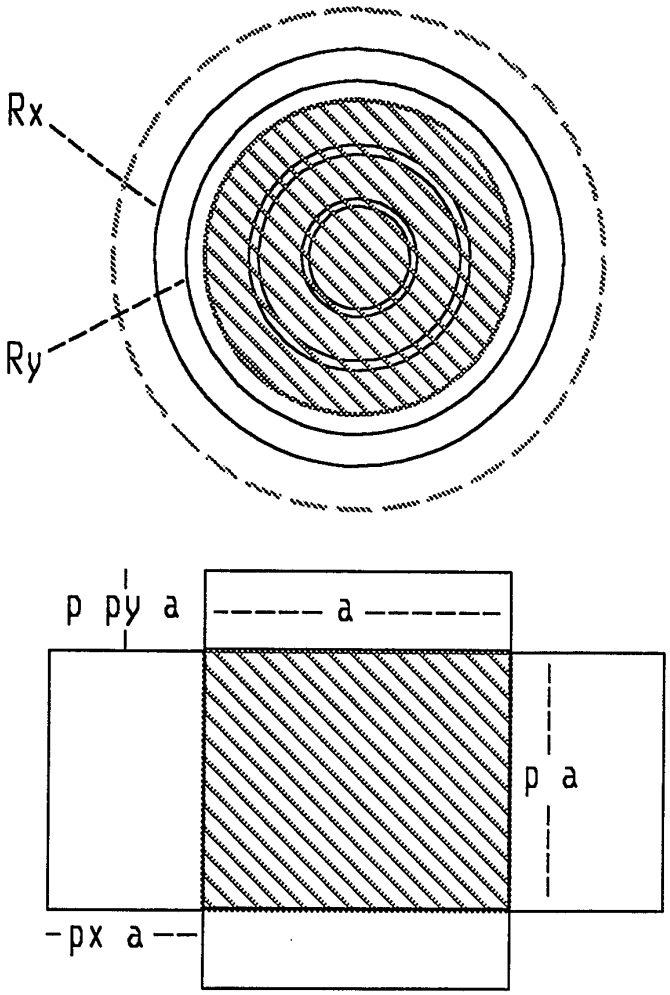
\includegraphics[width=.6\columnwidth]{mecs-geometry}
    \caption{Geometries of the absorber region and its vicinity in the super
        cell (top) and the diffusion solver mesh (bottom).
        The shaded and unshaded regions represent the homogenized absorber
        region and the adjacent non-absorber region, respectively.
        Retrieved from Fen et al. \cite{fen_modelling_1992}.}
    \label{fig:mecs-geometry}
\end{figure}

Figure \ref{fig:mecs-geometry} shows the 1D cylindrical super cell for the
transport solver on the top and the corresponding 2D Cartesian geometry for the
diffusion solver on the bottom. The four adjacent nodes in the Cartesian
geometry and their corresponding flux values are pairwise identical.

According to the mesh-centered geometry in CITATION, the leakage $L$ is
calculated as:
%
\begin{align}
  L =& \frac{F_y\left(\phi_x-\phi_a\right)}{\frac{\delta_x}{D_a}+
    \frac{\Delta_x}{D_o}} + \frac{F_x\left(\phi_y-\phi_a\right)}{
  \frac{\delta_y}{D_a}+\frac{\Delta_y}{D_o}} \label{eq:mecs}
  \shortintertext{where}
  \phi_x =& \mbox{ flux in the $x$-neighbor nodes,} \nonumber \\
  \phi_y =& \mbox{ flux in the $y$-neighbor nodes,} \nonumber \\
  \phi_a =& \mbox{ flux in the absorber node,} \nonumber \\
  F_y =& \mbox{ surface area to $y$-neighbor nodes} = 2pa, \nonumber \\
  F_x =& \mbox{ surface area to $x$-neighbor nodes} = 2a, \nonumber \\
  \delta_x =& \mbox{ distance from the absorber node center to the
    $x$-surface} = a/2, \nonumber \\
  \delta_y =& \mbox{ distance from the absorber node center to the
    $y$-surface} = pa/2, \nonumber \\
  \Delta_x =& \mbox{ distance from the $x$-surface to the $x$-neighbor node
    center} = p_x a/2, \nonumber \\
  \Delta_y =& \mbox{ distance from the $y$-surface to the $y$-neighbor node
    center} = p p_y a/2, \nonumber \\
  a, p, p_x, p_y =& \mbox{ geometric parameters of the CITATION mesh geometry
    (Figure \ref{fig:mecs-geometry}),} \nonumber \\
  D_a =& \mbox{ diffusion coefficient in the absorber node,} \nonumber \\
  D_o =& \mbox{ diffusion coefficient in the neighboring nodes.} \nonumber
\end{align}

In the original formulation by Scherer \& Neef \cite{scherer_determination_1976}, they chose to let
$D_a=D_o$. Taking leakage and flux values at $R_x$ and $R_y$ (figure \ref{fig:mecs-geometry}) from
the transport solver to be equal to the corresponding values in equation \ref{eq:mecs} yields a
value for $\phi_a$ which also represents the average flux in the absorber region. The equivalent
cross sections for each reaction type $i$ is then determined by matching reaction rates from the
transport calculation to the reaction rate as governed by diffusion theory as follows:
%
\begin{align}
  \Sigma_i =& \frac{A_i}{\phi_a V}
  \shortintertext{where}
  \Sigma_i =& \mbox{ macroscopic cross section of reaction type $i$,} \nonumber \\
  A_i =& \mbox{ reaction rate of reaction type $i$ from the transport calculation,} \nonumber \\
  V =& \mbox{ volume of the absorber region} = a^2 p.
\end{align}

Fen et al. \cite{fen_modelling_1992} later provided an updated formulation by assuming that the
cross sections are accurate and instead determined the equivalent diffusion coefficient from Eq.
\ref{eq:mecs} and the transport leakage and flux values as follows:
%
\begin{align}
  \frac{1}{D_a} =& 2p\frac{\phi_x-\phi_a}{L}+\frac{2}{p}\frac{\phi_y-\phi_a}{L}
    -\frac{p_x+p_y}{2D_o}+\sqrt{R}
  \shortintertext{where}
  R =& \left(2p\frac{\phi_x-\phi_a}{L}+\frac{2}{p}\frac{\phi_y-\phi_a}{L}+
  \frac{p_x+p_y}{2D_o}\right)^2+4p\left(p_y-p_x\right)\frac{\phi_x-\phi_a}{L}
  \frac{1}{D_o} \nonumber
\end{align}

As illustrated by the implementation in CITATION, \gls{MECS} requires considerable user input on
the super cell configuration to ensure that leakage rates of the transport solution are equivalent
to the leakage rates of the subsequent diffusion solution. This procedure also places some
constraints on the location and size of the absorber node that can be inconsistent with the
nodalization of the rest of the reactor geometry \cite{ougouag_transport_2010}. \gls{MECS} is also
incompatible with reactor geometries which contain control rods that are too close to each other
such that there is not enough distance in between to define neighboring nodes where
flux-equivalence is assumed. Nevertheless, \gls{MECS} has been widely used within the \gls{VSOP}
suite of codes (which contains CITATION) and has been shown to be effective in a number of
\gls{HTGR} studies \cite{fen_modelling_1992, reitsma_evaluating_2003, mulder_neutronics_2020}.

\subsubsection{Response-Based Methods}

Similar to the \gls{MECS}, \textit{response-based methods} rely on response-function-based
transport methods to resolve the flux around absorber regions. In this context, coarse mesh/nodal
response functions relate quantities of interest of an individual node to input values from its
neighboring nodes. For instance, a response function may provide the average nodal flux and the
outgoing partial currents of a node in response to a given set of incident
partial fluxes from its neighboring nodes \cite{ougouag_transport_2010}. Transport solutions are
used to generate sets of response functions characterizing individual coarse meshes which contain
absorber regions. These response functions can be used directly or indirectly as modified boundary
conditions to accurately capture the effects of control rods on the global flux solution.

%% Delete paragraph below if not relevant
%The response-based methods described here are closely related to response-function-based transport
%methods \cite{mosher_incident_2006}, in which every node is characterized by a set of response
%functions as opposed to only generating response functions for nodes that contain absorber regions.
%The main difference lies in the accuracy and/or presence of higher order expansions of the neutron
%phase space distribution in response-function-based transport methods compared to similar
%diffusion methods. Accordingly, response-function-based transport calculations are more accurate as
%they capture more information from the reference heterogeneous transport solution for each node.

Fen et al. \cite{fen_modelling_1992} developed the \gls{RMM} which generates modified boundary
conditions from response functions to treat absorber nodes in whole core diffusion calculations.
The response functions relate the incident partial current on one face of the node to the resultant
outgoing partial currents on all four faces of the same node. To be more precise, each incident
partial current of each neutron energy group on each face may contribute to the outgoing partial
current of any energy group on any face of the same node. The following equation for the response
matrix $A$ encapsulates the response values to be generated from the \gls{RMM}:
%
\begin{align}
  A^{jk}_{nm} =& \frac{J^{+j}_n}{J^{-k}_m} \mbox{ for } j,k=1...G \mbox{ and } n,m=1...N
  \label{eq:rmm} \\
  \shortintertext{where}
  A =& \mbox{ response matrix,} \nonumber \\
  N =& \mbox{ number of spatial intervals along the perimeter of the absorber node,} \nonumber \\
  J^{-k}_m =& \mbox{ incident partial current in energy group $k$ at spatial interval $m$,}
    \nonumber \\
  J^{+j}_n =& \mbox{ outgoing partial current in energy group $j$ at spatial interval $n$}
    \nonumber \\
  &\mbox{ in response to $J^{-k}_m$.} \nonumber
\end{align}

The \gls{RMM} compares favorably against the \gls{MECS} because it captures non-isotropic flux
effects arising from the non-central control rod location within the reactor core
\cite{fen_modelling_1992}. The \gls{RMM} also does not require
meticulously tuning of thick adjacent nodes to obtain equivalent fluxes to apply the \gls{MECS}.
However, both \gls{RMM} and \gls{MECS} involve precalculation procedures which must be rerun if the
absorber region is subjected to significant changes.

Rahnema et al. \cite{rahnema_advanced_2011} later developed an \gls{IDT} method which embeds the
transport correction for absorber regions in the full-core nodal diffusion calculation. Instead of
modified boundary conditions, the \gls{IDT} method generates coupling coefficients which are
morphologically identical to those used in nodal diffusion methods. The response region, which
contains the absorber region, is further subdivided into several nodes. The transport correction
relies on higher order spatial and angular response moments to maintain detailed responses between
adjacent response nodes. Changes in the response region can be modeled by swapping out response
nodes without having to rerun the transport solver to generate new coupling coefficients. The
intra-response region calculations were iteratively coupled to the full-core diffusion calculations
to avoid introducing extra off-diagonal terms which would increase the solve time of an otherwise
tri-diagonal system of nodal diffusion equations. In several verification studies of static
\gls{HTGR} core configurations, the \gls{IDT} method produced similar eigenvalue and flux
distribution results \cite{rahnema_advanced_2011} as the \gls{RMM}. However, they did not
demonstrate the response region swapping that the \gls{IDT} was designed for.

\subsubsection{Ronen Method}

Ronen \cite{ronen_accurate_2004} postulated an alternative formulation for diffusion coefficients
based on neutron currents from transport calculations.
Fick's law of diffusion is valid under three assumptions: the neutron flux gradient is small, the
absorption-to-scattering ratio is small, and scattering sources are isotropic. Therefore, diffusion
theory fails for anisotropic fluxes in and near absorber regions. The Ronen method proposes using
the integral form of the transport equation to derive transport operators for the neutron current
and substituting the values into Fick's first law of diffusion (Eq. \ref{eq:fick}) to obtain
space-dependent diffusion coefficients as follows:
%
\begin{align}
  D(\vec{r},E) =& -\frac{J_{tr}(\vec{r},E)}{\nabla \phi(\vec{r},E)}
  \label{eq:ronen}
  \shortintertext{where}
  J_{tr} =& \mbox{ transport-derived neutron current.} \nonumber
\end{align}

In doing so, the Ronen method provides pointwise corrections to the diffusion equation which
overcome the small flux gradient limitation. Tomatis \& Dall'Osso \cite{tomatis_application_2011}
numerically implemented the Ronen method for a 1D homogeneous slab with two energy groups and
isotropic scattering. Instead of using Eq. \ref{eq:ronen} which showed instabilities near flat flux
regions where the denominator approaches zero, they calculated corrections to the diffusion
coefficients at cell interfaces using the difference between the transport- and diffusion-derived
currents as follows:
%
\begin{align}
  \delta D(x_{i+1/2},E) =& -\delta J(x_{i+1/2},E) \frac{(\Delta x_{i+1}+\Delta x_i)/2}{
  \phi(x_{i+1},E)-\phi(x_i,E)}
  \shortintertext{where}
  x_i =& \mbox{ $i$-th spatial interval,} \nonumber \\
  \delta J(x,E) =& J_{tr}(x,E) - J_D(x,E), \nonumber \\
  \Delta x_i =& \mbox{ size of $i$-th spatial interval.} \nonumber
\end{align}

They derived expressions for the transport operators for $J_{tr}$ in terms of exponential integral
functions and Legendre expansions of the angular flux.
Gross et al. \cite{gross_high-accuracy_2020} extended the derivation of the transport operators to
handle 1D heterogeneous problems in the form of fuel assemblies with fuel, water, and fuel+absorber
regions. Tomatis et al. \cite{tomatis_ronen_2021} developed new numerical implementations for 1D
slab, cylindrical, and spherical geometries by employing probabilistic treatments from the
\gls{CPM} \cite{lewis_computational_1984} for the transport operators. The authors also implemented
a solver acceleration scheme which helped with the poor convergence rate observed in the earlier
studies \cite{tomatis_application_2011, gross_high-accuracy_2020}.

The results from all three studies showed improvements in flux solutions with the Ronen method over
pure diffusion solvers in all of the test cases, particularly for a 1D heterogeneous
\gls{BWR}-based problem with isotropic scattering and strong absorption cross sections
\cite{gross_high-accuracy_2020}. The error in reactivity values for three different \gls{BWR}
configurations differed from the reference $S_16$ transport calculations by at most 62 pcm after
one hundred iterations ($1$ pcm $=10^{-5}$) . However, the demonstrations were limited to simple
1D geometries. Although the authors provided derivations for anisotropic scattering, their test
cases incorporated only isotropic scattering. The derivation of semi-analytic transport operators
for more complex reactor geometries would be a much more complicated endeavor. Furthermore, without
an accompanying solver acceleration scheme, poorly converged solutions retained significant
discrepancies near material interfaces and vacuum boundaries.

\subsubsection{Averaged Eddington Factors and High-Order Empirical Diffusion Coefficients}

In a similar vein, Pounders \& Rahnema developed two separate methods for generating
space-dependent diffusion coefficients \cite{pounders_diffusion_2009}. Both methods come with the
same caveat in requiring a priori knowledge of the flux and current. The first method, called the
\gls{AEF} method, relies on the Eddington factor, which is defined as the second angular moment of
the angular flux normalized by its zeroth moment. In 1D, the Eddington factor is given as:
%
\begin{align}
  E_g(z) =& \frac{\int^1_{-1} \mu^2\psi(z,\mu)d\mu}{\int^1_{-1} \psi(z,\mu)d\mu}
\end{align}
%
The $g$ subscript denotes the discrete neutron group index of the multigroup diffusion equations
obtained from discretizing the continuous energy variable as described in Section
\ref{sec:challenges-control-rod}. The Eddington factor features in the fist angular moment of the
1D multigroup transport equations, obtained by multiplying the transport equation throughout by
$\mu=\cos\theta$ and integrating over $\mu=-1$ to $\mu=1$:
%
\begin{align}
  \frac{d\left[E_g(z)\phi_g(z)\right]}{dz} + \Sigma_{t,g}(z)J_g(z) =& \sum^G_{g'=1}
  \Sigma^{g'\rightarrow g}_{s1}(z)J_{g'}(z) \label{eq:bte-1st-mom}
  \shortintertext{where}
  \Sigma^{g'\rightarrow g}_{s1} =& \int^1_{-1} \mu \Sigma_s d\mu \nonumber
\end{align}
%
Assuming the Eddington factor varies slowly in space, we can approximate Eq. \ref{eq:bte-1st-mom}
as:
%
\begin{align}
  E_g(z)\frac{d\bar{\phi}_g(z)}{dz} + \Sigma_{t,g}(z)\bar{J}_g(z) =& \sum^G_{g'=1}
  \Sigma^{g'\rightarrow g}_{s1}(z)\bar{J}_{g'}(z) \mbox{ for } z \in V_i \label{eq:bte-1st-est}
  \shortintertext{where}
  V_i =& \mbox{ a subvolume of the system domain.}
\end{align}
The overbars distinguish the approximate solutions of Eq. \ref{eq:bte-1st-est} from the true
solution of Eq. \ref{eq:bte-1st-mom}. From Eq. \ref{eq:bte-1st-est}, the diffusion coefficient can
be defined as:
%
\begin{align}
  D_g(z) = E_g(z)\left[\Sigma_{t,g}(z)-\sum^g_{g'=1}\Sigma^{g'\rightarrow g}_{s1}(z)
  \frac{\bar{J}_{g'}(z)}{\bar{J}_g(z)}\right]^{-1} \label{eq:diffcoef-edd}
\end{align}
By further assuming that the Eddington factors are piecewise constant in each subvolume $V_i$, the
averaged Eddington factor $E^i_g$ can be evaluated as:
%
\begin{align}
  E^i_g =& \frac{E_g(z_{i+1})\phi_g(z_{i+1})-E_g(z_i)\phi_g(z_i)}{\bar{\phi}_g(z_{i+1})-
  \bar{\phi}_g(z_i)}
  \shortintertext{where}
  z_{i+1} =& \mbox{ upper bound of subvolume $V_i$,} \nonumber \\
  z_i =& \mbox{ lower bound of subvolume $V_i$.} \nonumber
\end{align}
%
The diffusion coefficient from Eq. \ref{eq:diffcoef-edd} can then be calculated as:
%
\begin{align}
  D^{AEF}_g(z) =& E^i_g\left[\hat{\Sigma}_{t,g}-\sum^G_{g'=1}\hat{\Sigma}^{g'\rightarrow g}_{s1}
  \frac{\hat{J}_{g'}}{\hat{J}_g}\right]^{-1}
  \shortintertext{where}
  \hat{\Sigma}_{t,g} =& \frac{\int_{V_i}\Sigma_{t,g}(z)J_g(z)dz}{\int_{V_i}\bar{J}_g(z)dz},
  \nonumber \\
  \hat{\Sigma}^{g'\rightarrow g}_{s1} =& \frac{\int_{V_i}\Sigma^{g'\rightarrow g}_{s1}(z)J_{g'}(z)
  dz}{\int_{V_i}\bar{J}_{g'}(z)dz}, \nonumber \\
  \hat{J}_g =& \int_{V_i} \bar{J}_g(z)dz. \nonumber
\end{align}

The second method employs a much simpler premise in that Fick's law is assumed to be accurate with
high-order empirical diffusion coefficients that are to be determined. Given a known transport
solution, the following integration holds for a small homogeneous volume $V_i$:
%
\begin{align}
  \frac{1}{V_i}\int_{V_i}J_g(z)dV =& -\frac{1}{V_i}\int_{V_i}D_g(z)\frac{d\phi_g(z)}{dz}dV.
\end{align}
%
Taking $D_g$ to be constant in $V_i$, we may apply divergence theorem to obtain
%
\begin{align}
  \bar{J}_gV_i =& -D^i_g\int_{\partial V_i} \phi_g(z)dA
  \shortintertext{where}
  \bar{J}_g =& \mbox{ average current in $V_i$,} \nonumber \\
  \partial V_i =& \mbox{ bounding surface of $V_i$.} \nonumber
\end{align}
%
Rearranging the terms, we may obtain the empirical diffusion coefficient formulation from the
transport-derived flux and current as follows:
%
\begin{align}
  D^i_g =& -\frac{\left(z_{i+1}-z_i\right) \bar{J}_g}{\left[\phi_g(z_{i+1})-\phi_g(z_i)\right]}
\end{align}
%
Both \gls{AEF} and empirical methods require the respective subvolumes $V_i$ to be small enough
for the assumptions of constant Eddington factors and diffusion coefficients to hold within $V_i$.

Both methods performed much better than with conventional diffusion coefficients derived using the
$P_1$ approximation method. For the same 1D heterogeneous \gls{BWR} problem demonstrating the prior
Ronen method \cite{gross_high-accuracy_2020} but with anisotropic scattering, the reactivity errors
were around 10 pcm after eliminating errors associated with energy group condensation. The error
values compare favorably with the 16-68 pcm error with the $P_1$ method. The \gls{AEF} and
empirical methods also reproduced the flux distributions better with a maximum pointwise error of
2\% as opposed to 5\% from the $P_1$ method. Similar to the Ronen method, the \gls{AEF} and
empirical methods introduce pointwise corrections with information from transport methods. However,
the present methods require a priori knowledge of the true solution or otherwise accurate estimates
from transport methods, whereas the Ronen method relies on analytical transport operators which use
diffusion flux estimates from the previous iteration to update the flux solution. Nevertheless, the
\gls{AEF} and empirical methods provide the foundation for further development of practical,
self-closing transport correction techniques.

\subsubsection{General Equivalence Theory and Superhomogenization Method}

As mentioned in Section \ref{sec:challenges-control-rod}, coarse-mesh and nodal methods homogenize
heterogeneities in reactor geometries to reduce computational costs of running full-core
simulations. Equivalence techniques which reduce spatial homogenization error are also effective
for accurately modeling the worths of control rods within fuel assemblies. The \gls{GET}
\cite{koebke_new_1980, smith_nodal_1983} and \gls{SPH} \cite{kavenoky_sph_1978,
hebert_consistent_1991} methods represent the most widely used equivalence methods for improving
the performance of diffusion calculations in homogenized \gls{LWR} models. Both methods involve
deriving additional homogenization parameters from single-assembly transport calculations with
reflective boundary conditions. Since the transport calculation step is already a prerequisite step
for generating homogenized group constants, the equivalence methods are simple to implement and
impose reasonably small additional computational costs.

Koebke \cite{koebke_new_1980} first proposed abandoning continuous surface fluxes in favor of
preserving net surface currents through discontinuity factors. Smith \cite{smith_assembly_1986}
later extended this concept for assembly-homogenized calculations. The discontinuity factors are
calculated for each face of the homogenized region to preserve volumetric reaction rates and
surface neutron currents. The discontinuity factors are calculated as follows:
%
\begin{align}
  DF =& \frac{\phi^{het,sur}}{\phi^{hom,sur}}
  \shortintertext{where}
  DF =& \mbox{ discontinuity factor,} \nonumber \\
  \phi^{het,sur} =& \mbox{ surface flux of the region from the heterogeneous calculation,}
  \nonumber \\
  \phi^{hom,sur} =& \mbox{ surface flux of the region from the homogeneous calculation.}
  \nonumber
\end{align}
%
\gls{GET} was later extended for fine mesh calculations \cite{yamamoto_cell_2004} which refers to
cell-level homogenization; each fuel cell in an assembly, consisting of the fuel pellet, cladding,
and moderator, is individually homogenized as opposed to lumping together the entire assembly.

On the other hand, the \gls{SPH} method, first proposed by Kavenoky \cite{kavenoky_sph_1978} for
irregular lattices and later applied as a cell-homogenization technique by Hebert
\cite{hebert_consistent_1991}, introduces correction factors to homogeneous cross sections as
follows:
%
\begin{align}
  \tilde{\Sigma}^{hom}_k =& \mu_k \Sigma^{hom}_k
  \shortintertext{where}
  \tilde{\Sigma}^{hom}_k =& \mbox{ \gls{SPH}-corrected homogeneous cross section for region $k$,}
  \nonumber \\
  \mu_k =& \mbox{ \gls{SPH} correction factor for region $k$,} \nonumber \\
  \Sigma^{hom}_k =& \mbox{ uncorrected homogeneous cross section for region $k$.} \nonumber
\end{align}
%
The \gls{SPH} factor is calculated as follows:
%
\begin{align}
  \mu_k =& \frac{\bar{\phi}^{het}_k}{\phi^{hom}_k}
  \shortintertext{where}
  \bar{\phi}^{het}_k =& \mbox{ average flux in region $k$ from the heterogeneous calculation,}
  \nonumber \\
  \phi^{hom}_k =& \mbox{ average flux in region $k$ from the homogeneous calculation}
  \nonumber \\
                & \mbox{ with \gls{SPH}-corrected cross sections.} \nonumber
\end{align}

Both \gls{GET} and the \gls{SPH} method are designed to preserve reaction rates at the assembly
level \cite{yamamoto_cell_2004}. Given that the \gls{SPH} method introduces only one correction
factor per cell, it only preserves the average net current across all surfaces as opposed
to the net current at each surface with \gls{GET}. Similarly, the isotropic nature of \gls{SPH}
factors lead to worse pin-power estimates near control rods and reflectors compared to \gls{GET}.
However, the \gls{SPH} method is simpler to implement in the diffusion solver as the \gls{SPH}
factors can be precombined with the cross sections to generate \gls{SPH}-corrected cross sections.
\gls{GET} requires diffusion solvers which allow for flux discontinuities at the interfaces.
Furthermore, \gls{GET} requires more memory to store up to six discontinuity factors, one for each
mesh surface, in 3D calculations.

Modeling control rods in full-core calculations with the \gls{SPH} method or \gls{GET} provides
better estimates of the multiplication factor and the flux distribution than reference diffusion
solutions. In this regard, the correction factors do not distinguish between errors arising from
homogenization or the diffusion approximation. However, the improved solutions, especially with the
\gls{SPH} method, can still deviate significantly from reference transport calculations. A super
cell, similar to the one adopted by \gls{MECS}, can be used to reduce errors within and near
control rod cells \cite{ortensi_newton_2018}.
